\chapter{Ergebnisse}
\label{sec:ergebnisse}

Im folgenden Protokollabschnitt werden die Versuchsergebnisse der Versuchsdurchführung präsentiert.
\vspace*{-3.5mm}

\section{Sedimentationsverhalten}

% pgf diagramm3 START
\begin{figure}[h!]
	\begin{center}
		%\resizebox{0.8\textwidth}{!}{
		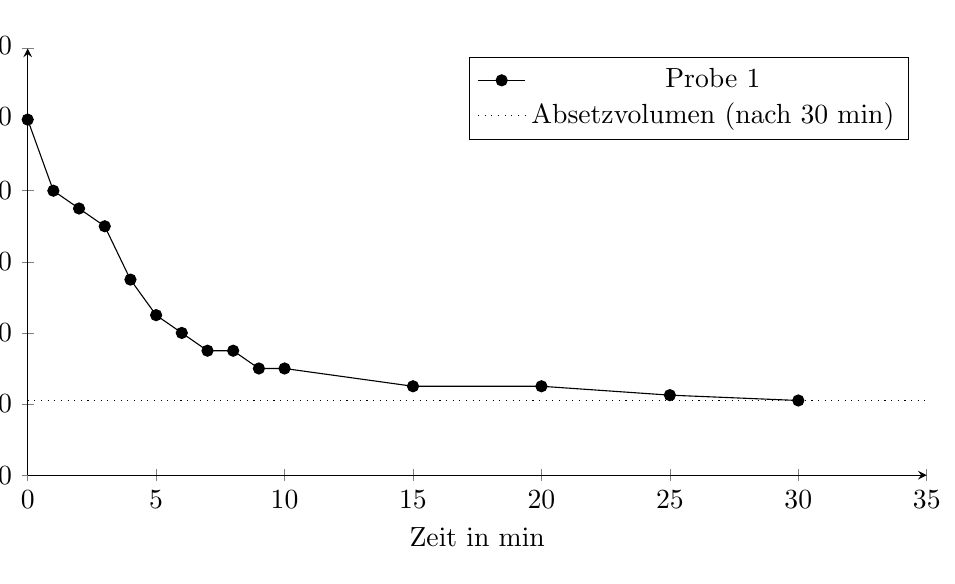
\begin{tikzpicture}[trim axis left, trim axis right]
		\begin{axis}[
		axis lines = left,
		width = 13cm,
		height = 7cm,
		xmin = 0,
		xmax = 35,
		ymin = 0,
		ymax = 1200,
		ylabel={Absetzvolumen in $\si{\milli \liter}$},
		y label style={at={(-0.03,0.5)}},
		xlabel={Zeit in min},
		]
		\addplot[black,mark=*,text mark as node=true,point meta=explicit symbolic,nodes near coords]
		coordinates {(0, 1000) (1, 800) (2, 750) (3, 700) (4, 550) (5, 450) (6,400) (7,350) (8,350) (9,300) (10,300) (15,250) (20,250) (25,225)(30,210)};
		
		\addplot[no markers, dotted] coordinates {(0,210)(35,210)};
		
		\legend{Probe 1, Absetzvolumen (nach 30 min)}
		\end{axis}
		\end{tikzpicture}
		%	}
		\caption{Sedimentationskurve für Abwasserprobe 1}
		\label{dia:sedimentation_1}
	\end{center}
\end{figure}
\FloatBarrier
% pgf diagramm3 ENDE

\vspace*{10mm}

% pgf diagramm3 START
\begin{figure}[h!]
	\begin{center}
		%\resizebox{0.8\textwidth}{!}{
		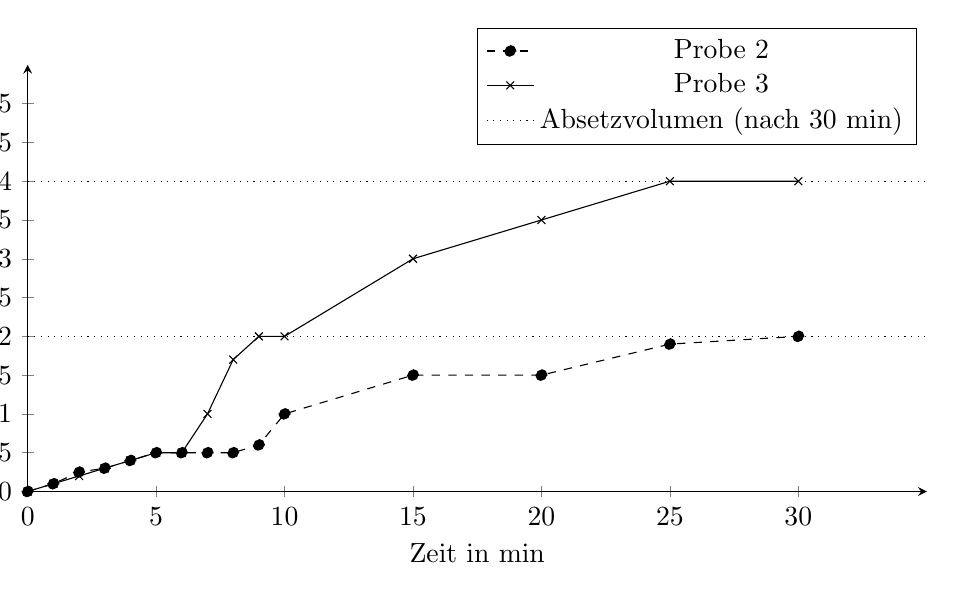
\begin{tikzpicture}[trim axis left, trim axis right]
		\begin{axis}[
		axis lines = left,
		width = 13cm,
		height = 7cm,
		xmin = 0,
		xmax = 35,
		ymin = 0,
		ymax = 5.5,
		ytick = {0,0.5,...,5},
		xtick = {0,5,...,30},
		ylabel={Absetzvolumen in $\si{\milli \liter}$},
	%	y label style={at={(-0.03,0.5)}},
		xlabel={Zeit in min},
		legend style={at={(0.5,0.95)},anchor=west}
		]
		
		\addplot[black,mark=*,text mark as node=true,point meta=explicit symbolic,nodes near coords, dashed]
		coordinates {(0, 0) (1, 0.1) (2, 0.25) (3, 0.3) (4, 0.4) (5, 0.5) (6,.5) (7,.5) (8,.5) (9,.6) (10,1) (15,1.5) (20,1.5) (25,1.9)(30,2)};
		
		\addplot[black,mark=x,text mark as node=true,point meta=explicit symbolic,nodes near coords]
		coordinates {(0, 0) (1, 0.1) (2, 0.2) (3, 0.3) (4, 0.4) (5, .5) (6,.5) (7,1.0) (8,1.7) (9,2) (10,2.0) (15,3) (20,3.5) (25,4.)(30,4)};
		
		\addplot[no markers, dotted] coordinates {(0,4)(35,4)};
		
		\addplot[no markers, dotted] coordinates {(0,2)(35,2)};
		
		\legend{Probe 2, Probe 3, Absetzvolumen (nach 30 min)}
		\end{axis}
		\end{tikzpicture}
		%	}
		\caption{Sedimentationskurve für Abwasserproben 2 und 3}
		\label{dia:sedimentation_12}
	\end{center}
\end{figure}
\FloatBarrier
% pgf diagramm3 ENDE

\newpage

\section*{Absetzvolumen}

%Tabelle START
\vspace*{-2.5mm}
\renewcommand{\arraystretch}{1.2}
\begin{table}[h!]
	%	\begin{adjustwidth}{-2cm}{-2cm} 
	%	\begin{center}
	\centering
	\caption{Messwerte für abfiltrierbare Stoffe}
	\label{tab:absetzvol}
	%	\resizebox{19cm}{!}{
	\begin{tabulary}{1.7\textwidth}{L|CCC}
		\hline
		& \textbf{Probe 1 $\boldsymbol{\left[\si{\milli \liter \per \liter}\right]}$}  & \textbf{Probe 2 $\boldsymbol{\left[\si{\milli \liter \per \liter}\right]}$} & \textbf{Probe 3 $\boldsymbol{\left[\si{\milli \liter \per \liter}\right]}$}  \\ 
		\hline
		\textbf{Absetzvolumen (nach 30 min)}&  210 	& 2 	& 4\\
		\hline
	\end{tabulary}
	%	}
	%	\end{center}
	%	\end{adjustwidth}
\end{table}
\FloatBarrier
\vspace*{-2.5mm}

%Tabelle Ende

\section{Trockensubstanz TS}
Beispielrechnung für Probe 1
\begin{flalign}
	m_{\text{Filterkuchen}}		&= m_{\text{Filterkuchen+Filter}}-m_{\text{Filter (trocken)}}\\
	m_{\text{Filterkuchen,1}}	&= \SI{0,611}{\gram}-\SI{0,487}{\gram}\\
								&=\underline{ \SI{0,124}{\gram}}\\[8pt]
	c_{\text{filtrierbar}} 		&= \frac{m_{\text{Filterkuchen}}}{V_{\text{Probe}}}\\[2mm]
	c_{\text{filtrierbar,1}} 	&= \frac{m_{\text{Filterkuchen,1}}}{V_{\text{Probe 1}}}\\[2mm]
								&= \frac{\SI{0,124}{\gram}}{\SI{94}{\milli \liter}}\\
								&= \SI{0.0013191489}{\gram\per \milli \liter} \approx \underline{\underline{\SI{1,32}{ \gram \per \liter}}}
\end{flalign}

%Tabelle START
\vspace*{-2.5mm}
\renewcommand{\arraystretch}{1.2}
\begin{table}[h!]
%	\begin{adjustwidth}{-2cm}{-2cm} 
	%	\begin{center}
	\centering
	\caption{Messwerte für abfiltrierbare Stoffe}
	\label{tab:filter}
%	\resizebox{19cm}{!}{
	\begin{tabulary}{1.7\textwidth}{L|C|CCC}
		\hline
		 & \textbf{Maßeinheit}&	\textbf{Probe 1} & \textbf{Probe 2} & \textbf{Probe 3}  \\ 
		\hline
	 	\textbf{Probenvolumen}& $\boldsymbol{\left[\si{\milli \liter}\right]}$ & 94 	& 300 	& 100\\
		\textbf{Masse Filter (trocken)} &  $\boldsymbol{\left[\si{\gram}\right]}$ & 0,487 & 0,465 & 0,497\\
		\textbf{Masse Filterkuchen + Filter }& $\boldsymbol{\left[\si{\gram}\right]}$	& 0,611 & 0,528 & 0,506\\
		\hline
		\textbf{Masse Filterkuchen} & $\boldsymbol{\left[\si{\gram}\right]}$& 0,124 &0,063&0,009\\
		\hline
		\textbf{Konzentration abfiltrierbare Stoffe}&$\boldsymbol{\left[\si{\gram \per \liter}\right]}$&1,32&0,21&0,09\\
		\hline
	\end{tabulary}
%	}
	%	\end{center}
%	\end{adjustwidth}
\end{table}
\FloatBarrier
\vspace*{-2.5mm}

%Tabelle Ende

\newpage

\section*{organische Trockensubstanz oTS}
Beispielrechnung für Probe 1\\
\textcolor{red}{Berechnung überarbeiten}
\begin{flalign}
m_{Filter,Glüh}	&= m_{Filter+Tiegel}-m_{Tiegel}\\
				&= \SI{35,7126}{\gram}-\SI{35,714}{\gram}\\
				&=\underline{ \SI{0,0014}{\gram}}\\[8pt]
m_{\text{oTS}}				&= m_{Filterkuchen}-(m_{\text{Tiegel+Probe}}-m_{\text{Tiegel}})-m_{Filter,Glüh}\\
m_{\text{oTS,1}}			&= \SI{0,124}{\gram}-(\SI{33,2209}{\gram}-\SI{33,2023}{\gram})-\SI{0,0014}{\gram}\\
							&= \underline{ \SI{0,104}{\gram}}\\[8pt]
c_{\text{oTS}} 				&= \frac{m_{\text{oTS}}}{V_{\text{Probe}}}\\[2mm]
c_{\text{oTS,1}} 			&= \frac{\SI{0,104}{\gram}}{\SI{94}{\milli \liter}}\\
							&= \SI{0.001106}{\gram\per \milli \liter} \approx \underline{\underline{\SI{1106}{\milli \gram \per \liter}}}\\
		w_{oTS}&=\frac{m_{oTS}}{m_{Filterkuchen}}\\
		w_{oTS,1}&=\frac{m_{oTS,1}}{m_{Filterkuchen}}\\
				&= \frac{\SI{0,104}{\gram}}{\SI{0,124}{\gram}}\\
				&\approx\underline{\underline{ \SI{84}{\percent}}}
\end{flalign}

%Tabelle START
\vspace*{-2.5mm}
\renewcommand{\arraystretch}{1.2}
\begin{table}[h!]
	%	\begin{adjustwidth}{-2cm}{-2cm} 
	%	\begin{center}
	\centering
	\caption{Messwerte für organische Trockensubstanz}
	\label{tab:ots}
	%	\resizebox{19cm}{!}{
	\begin{tabulary}{1.7\textwidth}{L|C|CCC}
		\hline
		& \textbf{Maßeinheit}&	\textbf{Probe 1} & \textbf{Probe 2} & \textbf{Probe 3}  \\ 
		\hline
		\textbf{Probenvolumen}& $\boldsymbol{\left[\si{\milli \liter}\right]}$ & 94 	& 300 	& 100\\
		\textbf{Masser Filter (verglüht)} & $\boldsymbol{\left[\si{\milli \gram}\right]}$ & \SI{0,0014}{\gram}&\SI{0,0014}{\gram}&\SI{0,0014}{\gram}\\
		\textbf{Masse Tiegel (leer)} &  $\boldsymbol{\left[\si{\gram}\right]}$ & 33,2023 & 31,0858 & 34,0671\\
		\textbf{Masse Tiegel (voll)}& $\boldsymbol{\left[\si{\gram}\right]}$	& 33,2209 & 31,1029 & 34,0713\\
		\hline
		\textbf{Masse oTS} & $\boldsymbol{\left[\si{ \gram}\right]}$& 0,104 & 0,106 & 0,118\\
		\hline
		\textbf{Konzentration oTS}&$\boldsymbol{\left[\si{\milli \gram \per \liter}\right]}$& 1106 & 352 & 1184 \\
		\textbf{Massenanteil oTS an TS} & $\boldsymbol{\left[\%\right]}$&84&85&95\\
		\hline
	\end{tabulary}
	%	}
	%	\end{center}
	%	\end{adjustwidth}
\end{table}
\FloatBarrier
\vspace*{-2.5mm}
%Tabelle Ende

\section{Schlammvolumenindex SVI}
%Quelle Römpp \cite{Dr.ManfredNeupert.August2008}\\

Beispielrechnung für Probe 1
\begin{flalign}
	SVI		&= \frac{\varphi_{\text{Absetzvolumen nach 30 min}}}{c_{\text{filtrierbar}}}\\
	SVI_1	&= \frac{\varphi_{\text{Absetzvolumen nach 30 min},1}}{c_{\text{filtrierbar},1}}\\
			&= \frac{\SI{210}{\milli \liter \per \liter}}{\SI{1319}{\milli \gram \per \liter}}\\
			&= \SI{0.1592}{\milli \liter \per \milli \gram} = \underline{\underline{\SI{159,2}{\milli \liter \per \gram}}}
\end{flalign}
%Tabelle START
\vspace*{-2.5mm}
\renewcommand{\arraystretch}{1.2}
\begin{table}[h!]
	%	\begin{adjustwidth}{-2cm}{-2cm} 
	%	\begin{center}
	\centering
	\caption{SVI für die Abwasserproben 1 bis 3}
	\label{tab:svi}
	%	\resizebox{19cm}{!}{
	\begin{tabulary}{1.7\textwidth}{L|C|C|C}
		\hline
		& \textbf{Probe 1 $\boldsymbol{\left[\si{\milli \liter \per \gram}\right]}$}& \textbf{Probe 2 $\boldsymbol{\left[\si{\milli \liter \per \gram}\right]}$} & \textbf{Probe 3 $\boldsymbol{\left[\si{\milli \liter \per \gram}\right]}$}  \\ 
		\hline
		\textbf{$\boldsymbol{SVI}$}& 159,2 & 9,5 & 44,4 \\
		\hline
	\end{tabulary}
	%	}
	%	\end{center}
	%	\end{adjustwidth}
\end{table}
\FloatBarrier
\textcolor{red}{Werte für Probe 2 und Probe 3 sinnlos, das gar kein richtiger Schlamm mehr vorhanden ist}

\section{chemischer Sauerstoffbedarf CSB}
Verdünnung Probe 1 mit 1:1\\
Messbereich 0-1500 ml/l\\
2ml derr Analyselösung in Reagenz mit Schwefelzeug gegeben \\

Berechnung CSB für Probe 1 aus 1:1 verdünnter Lösung, sprich Hälfte Probe Hälfte Wasser
\begin{flalign}
\frac{c_{\text{Probe 1}}}{c_{\text{Probe 1 (verdünnt)}}}  	&= \frac{2}{1} \\
c_{\text{Probe 1}}											&= 2*c_{\text{Probe 1 (verdünnt)}}\\
															&= 2*\SI{575}{\milli \gram \per \liter} \\
															&= \underline{\underline{\SI{1150}{\milli \gram \per \liter}}}
\end{flalign}
%Tabelle START
\vspace*{-8.5mm}
\renewcommand{\arraystretch}{1.2}
\begin{table}[h!]
	%	\begin{adjustwidth}{-2cm}{-2cm} 
	%	\begin{center}
	\centering
	\caption{Messwerte für den chemischen Sauerstoffbedarf für die Abwasserproben 1 bis 3}
	\label{tab:csb}
	%	\resizebox{19cm}{!}{
	\begin{tabulary}{1.7\textwidth}{L|CC|C|C}
		\hline
		& \textbf{Probe 1 (verdünnt) $\boldsymbol{\left[\si{\milli \gram \per \liter}\right]}$}  &\textbf{Probe 1 $\boldsymbol{\left[\si{\milli \gram \per \liter}\right]}$}& \textbf{Probe 2 $\boldsymbol{\left[\si{\milli \gram \per \liter}\right]}$} & \textbf{Probe 3 $\boldsymbol{\left[\si{\milli \gram \per \liter}\right]}$}  \\ 
		\hline
		\textbf{$\boldsymbol{CSB}$}& 575 & 1150 & 486 & 221 \\
		\hline
	\end{tabulary}
	%	}
	%	\end{center}
	%	\end{adjustwidth}
\end{table}
\FloatBarrier

\vspace*{-2.5mm}

\section[biologischer Sauerstoffbedarf BSB$_5$]{biologischer Sauerstoffbedarf BSB$\boldsymbol{_5}$}
Plätze 4,5,6 belegt\\
Messbereich für Probe 1 und 2 = 0-700 mg/L mit 95ml\\
Messbereich für Probe 3 = 0-350 mg/L mit 160ml

%Tabelle START
\vspace*{-2.5mm}
\renewcommand{\arraystretch}{1.2}
\begin{table}[h!]
	%	\begin{adjustwidth}{-2cm}{-2cm} 
	%	\begin{center}
	\centering
	\caption{Messwerte für den biologischen Sauerstoffbedarf über 5 Tage für die Abwasserproben 1 bis 3}
	\label{tab:bsb}
	%	\resizebox{19cm}{!}{
	\begin{tabulary}{1.7\textwidth}{L|C|C|C}
		\hline
		& \textbf{Probe 1 $\boldsymbol{\left[\si{\milli \gram \per \liter}\right]}$}& \textbf{Probe 2 $\boldsymbol{\left[\si{\milli \gram \per \liter}\right]}$} & \textbf{Probe 3 $\boldsymbol{\left[\si{\milli \gram \per \liter}\right]}$}  \\ 
		\hline
		\textbf{$\boldsymbol{BSB_5}$}& 254 & 252 & 50 \\
		\hline
	\end{tabulary}
	%	}
	%	\end{center}
	%	\end{adjustwidth}
\end{table}
\FloatBarrier


\newpage

\section{Gegenüberstellung der Mindestanforderungen für das Einleiten kommunaler Abwässer in einen Vorfluter der GK 5 mit den Abwasserproben}
Die Referenzwerte der Mindestanforderungen für das Einleiten kommunaler Abwässer in den Vorfluter der Größenklasse 5 sind im Anhang von \cite[S. 29]{Skript} zu finden.
\vspace*{-2.5mm}
\renewcommand{\arraystretch}{1.2}
\begin{table}[h!]
	\centering
	\caption{Tabellarischer Vergleich der Messwerte mit den Mindestanforderungen für das Einleiten kommunaler Abwässer in den Vorfluter der GK 5}
	\label{tab_vgl}
	%\resizebox{10cm}{!}{
	\begin{tabulary}{1.2\textwidth}{l|C|C}
		\hline
		 & \textbf{$CSB$} $\boldsymbol{\left[\si{\milli\gram\per\liter}\right]}$ & \textbf{$BSB_5$} $\boldsymbol{\left[\si{\milli\gram\per\liter}\right]}$\\
		\hline
		\textbf{Grenzwert} & \textbf{75} & \textbf{15}  \\
		\hline
		Probe 1 & 575 & 254 \\
		Probe 2 & 486 & 252\\
		Probe 3 & 221 & 50\\
		\hline
	\end{tabulary}
	%}
\end{table}
\FloatBarrier

\begin{figure}[h!]
	\begin{tikzpicture}
	\selectcolormodel{gray}
	\begin{axis}[
	xbar=1pt,% space of 0pt between adjacent bars
	bar width=7,
	width=15cm,
	height=7cm,
	%minor y tick num=4,
	xmax=600,xmin=0,
	x tick label style={/pgf/number format/.cd,%
		scaled x ticks = false,
		set decimal separator={,},
		fixed},
	symbolic y coords={Probe 3,Probe 2,Probe 1,max. für GK 5},
	ytick=data,
	%legend style={at={(0.5,-0.15)},
	%	anchor=north,legend columns=-1},
	xtick={0,50,...,600},
	grid=major,
	xlabel=Gehalt in  \si{\milli\gram\per\liter},
	%enlargelimits=0.15,
	%postaction={pattern=north east lines}
	]
	%CSB
	\addplot[fill=black] coordinates {
		(575,Probe 1) (486,Probe 2) (221,Probe 3) (75,max. für GK 5)
	};
	%BSB5
	\addplot coordinates {
		(254,Probe 1) (252,Probe 2) (50,Probe 3) (15,max. für GK 5)
	};

	\legend{$CSB$,$BSB_5$}
	\end{axis}
	\end{tikzpicture}
	\caption{Vergleich mit Mindestanforderungen für das Einleiten kommunaler Abwässer in den Vorfluter der GK 5 für die Abwasserproben 1 bis 3}
	\label{Balkendiagramm}
\end{figure}
\FloatBarrier


\newpage

\section{Gegenüberstellung der durchschnittlichen Beschaffenheit von häuslichem Abwasser mit den Abwasserproben}

Um die Messwerte des Versuches mit häuslichem Abwasser gegenüberzustellen wird die Tabelle Tab. \ref{tab:komm} (siehe \cite[S. 29]{Skript}) genutzt.

\vspace*{0.5cm}
\renewcommand{\arraystretch}{1.2}
\begin{table}[h!]
	\centering
	\caption[Tabellenausschnitt zur durchschnittlichen Beschaffenheit von häuslichem Abwasser]{Tabellenausschnitt zur durchschnittlichen Beschaffenheit von häuslichem Abwasser \cite[S. 29]{Skript}}
	\label{tab:komm}
	%\resizebox{10cm}{!}{
	\begin{tabulary}{1.2\textwidth}{l|C|C|C|C}
	\textbf{Kriterium} 		& \textbf{Maßeinheit} 				&\multicolumn{3}{c}{\textbf{Belastungsgrad}}\\
	\hline
							&									& gering	& mittel & stark\\
	\hline
	Absetzbare Stoffe		&\si{\milli \liter \per \liter} 	& 2			& 6	 	 & 12\\
	Abfiltrierbare Stoffe	&\si{\milli \gram \per \liter} 		& 200		&500	 & 900\\
	$CSB$					&\si{\milli \gram \per \liter} 		& 300		&600	 & 1000\\
	$BSB_5$					&\si{\milli \gram \per \liter}		& 150		&300	 & 500\\
	\end{tabulary}
	%}
\end{table}
\FloatBarrier
\vspace*{1.5cm}

\begin{figure}[h!]
	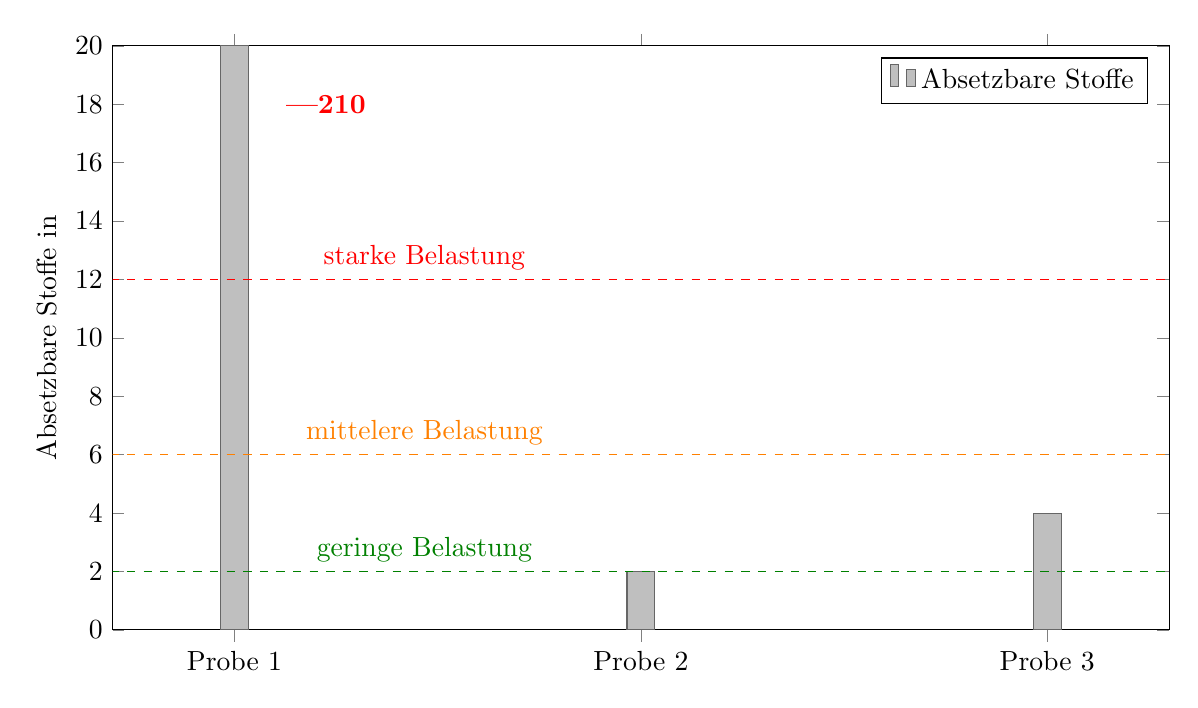
\begin{tikzpicture}
	\begin{axis}[
	%x tick label style={
	%	/pgf/number format/1000 sep=},
	xtick = data,
	ylabel=Absetzbare Stoffe in \si{\milli \liter \per \liter},
   	enlarge x limits=0.15,
	ybar,
	ymin = 0,
	ymax = 20,
	bar width=10pt,
	width=15cm,
	height=9cm,
	symbolic x coords={0,Probe 1, Probe 2,Probe 3,2,1},
	]
	\addplot[fill=gray!50,draw=black!60] coordinates {(Probe 1,20) (Probe 2,2) (Probe 3,4)
	};
	\addplot[green!50!black,sharp plot,update limits=false, dashed] 
	coordinates {(0,2) (1,2)} 
	node[above] at (axis cs:Probe 2,2) {\hspace*{-5.5cm}geringe Belastung
	};
	\addplot[orange,sharp plot,update limits=false, dashed] 
	coordinates {(0,6) (1,6)} 
	node[above] at (axis cs:Probe 2,6) {\hspace*{-5.5cm}mittelere Belastung
	};
	\addplot[red,sharp plot,update limits=false, dashed] 
	coordinates {(0,12) (1,12)} 
	node[above] at (axis cs:Probe 2,12) {\hspace*{-5.5cm}starke Belastung
	};
	\node[red] at (axis cs: Probe 2,18) {\hspace*{-8.cm}\textbf{---\SI{210}{\milli \liter \per \liter}}};
	\legend{Absetzbare Stoffe}
	\end{axis}
	\end{tikzpicture}
	\caption{Absetzbare Stoffe der Abwasserproben 1 bis 3}
	\label{dia:absetz}
\end{figure}
\FloatBarrier

\begin{figure}[h!]
	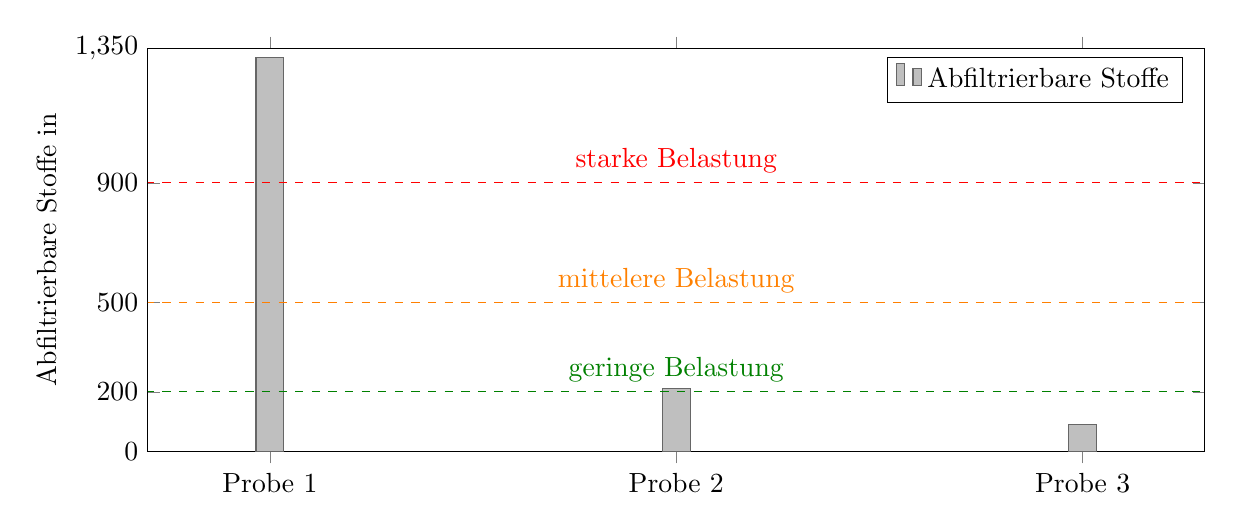
\begin{tikzpicture}
	\begin{axis}[
	%x tick label style={
	%	/pgf/number format/1000 sep=},
	xtick = data,
	ylabel=Abfiltrierbare Stoffe in \si{\milli \gram \per \liter},
	enlarge x limits=0.15,
	ybar,
	ymin = 0,
	ymax = 1350,
	ytick ={0,200,500,900,1350},
	bar width=10pt,
	width=15cm,
	height=6.7cm,
	symbolic x coords={0,Probe 1, Probe 2,Probe 3,2,1},
	]
	\addplot[fill=gray!50,draw=black!60] coordinates {(Probe 1,1319) (Probe 2,210) (Probe 3,90)
	};
	\addplot[green!50!black,sharp plot,update limits=false, dashed] 
	coordinates {(0,200) (1,200)} 
	node[above] at (axis cs:Probe 2,200) {geringe Belastung
	};
	\addplot[orange,sharp plot,update limits=false, dashed] 
	coordinates {(0,500) (1,500)} 
	node[above] at (axis cs:Probe 2,500) {mittelere Belastung
	};
	\addplot[red,sharp plot,update limits=false, dashed] 
	coordinates {(0,900) (1,900)} 
	node[above] at (axis cs:Probe 2,900) {starke Belastung
	};
	\legend{Abfiltrierbare Stoffe}
	\end{axis}
	\end{tikzpicture}
	\caption{Abfiltrierbare Stoffe der Abwasserproben 1 bis 3 (siehe Tab. \ref{tab:filter})}
	\label{dia:abfilt}
\end{figure}
\FloatBarrier

\begin{figure}[h!]
	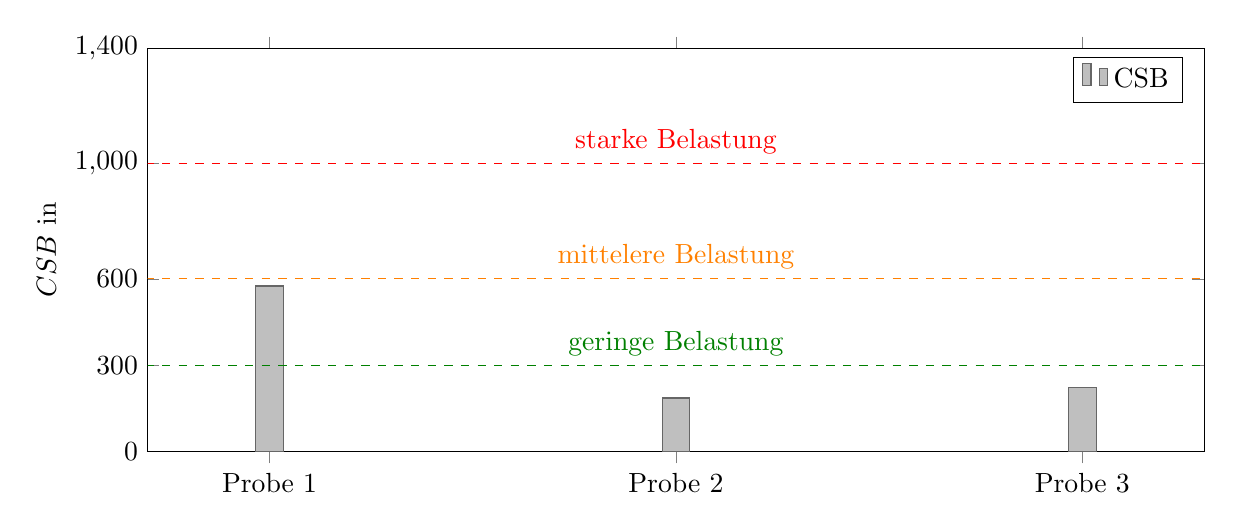
\begin{tikzpicture}
	\begin{axis}[
	%x tick label style={
	%	/pgf/number format/1000 sep=},
	xtick = data,
	ylabel=$CSB$ in \si{\milli \gram \per \liter},
	enlarge x limits=0.15,
	ybar,
	ymin = 0,
	ymax = 1400,
	ytick ={0,300,600,1000,1400},
	bar width=10pt,
	width=15cm,
	height=6.7cm,
	symbolic x coords={0,Probe 1, Probe 2,Probe 3,2,1},
	]
	%Daten der Proben
	\addplot[fill=gray!50,draw=black!60] coordinates {(Probe 1,575) (Probe 2,186) (Probe 3,221)
	};
	%Grenzen
	\addplot[green!50!black,sharp plot,update limits=false, dashed] 
	coordinates {(0,300) (1,300)} 
	node[above] at (axis cs:Probe 2,300) {geringe Belastung
	};
	\addplot[orange,sharp plot,update limits=false, dashed] 
	coordinates {(0,600) (1,600)} 
	node[above] at (axis cs:Probe 2,600) {mittelere Belastung
	};
	\addplot[red,sharp plot,update limits=false, dashed] 
	coordinates {(0,1000) (1,1000)} 
	node[above] at (axis cs:Probe 2,1000) {starke Belastung
	};
	\legend{CSB}
	\end{axis}
	\end{tikzpicture}
	\caption{Chemischer Sauerstoffbedarf (CSB) der Abwasserproben 1 bis 3}
	\label{dia:csb}
\end{figure}
\FloatBarrier

\begin{figure}[h!]
	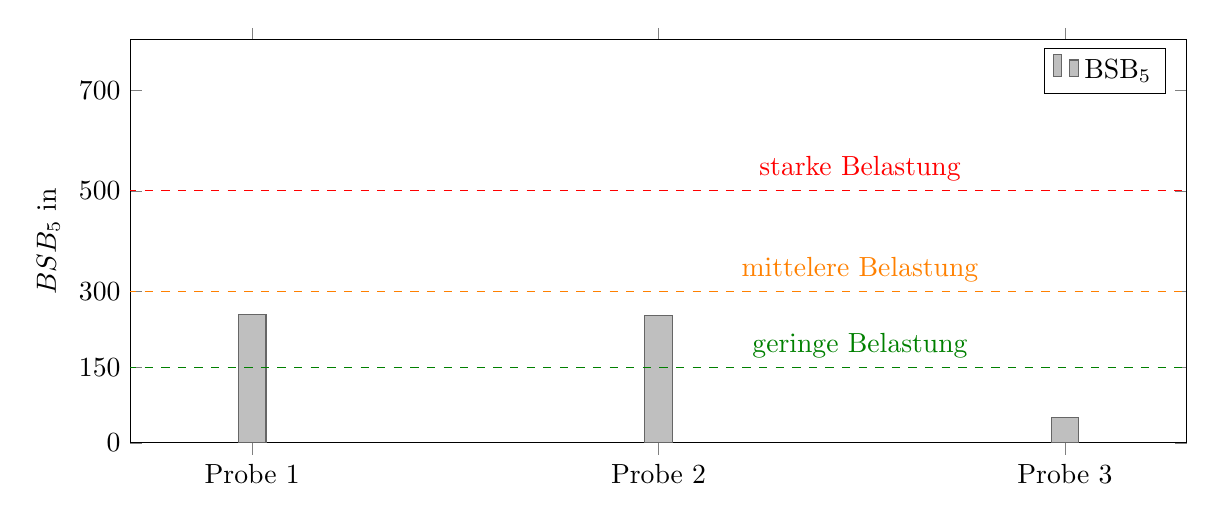
\begin{tikzpicture}
	\begin{axis}[
	%x tick label style={
	%	/pgf/number format/1000 sep=},
	xtick = data,
	ylabel=$BSB_5$ in \si{\milli \gram \per \liter},
	enlarge x limits=0.15,
	ybar,
	ymin = 0,
	ymax = 800,
	ytick ={0,150,300,500,700},
	bar width=10pt,
	width=15cm,
	height=6.7cm,
	symbolic x coords={0,Probe 1, Probe 2,Probe 3,2,1},
	]
	%Daten
	\addplot[fill=gray!50,draw=black!60] coordinates {(Probe 1,254) (Probe 2,252) (Probe 3,50)
	};
	%Linien
	\addplot[green!50!black,sharp plot,update limits=false, dashed] 
	coordinates {(0,150) (1,150)} 
	node[above] at (axis cs:Probe 2,150) {\hspace*{5cm} geringe Belastung
	};
	\addplot[orange,sharp plot,update limits=false, dashed] 
	coordinates {(0,300) (1,300)} 
	node[above] at (axis cs:Probe 2,300) {\hspace*{5cm} mittelere Belastung
	};
	\addplot[red,sharp plot,update limits=false, dashed] 
	coordinates {(0,500) (1,500)} 
	node[above] at (axis cs:Probe 2,500) {\hspace*{5cm} starke Belastung
	};
	\legend{BSB$_5$}
	\end{axis}
	\end{tikzpicture}
	\caption{Biochemischer Sauerstoffbedarf über 5 Tage (BSB$_5$) der Abwasserproben 1 bis 3}
	\label{dia:bsb}
\end{figure}
\FloatBarrier

